% !TEX encoding = IsoLatin2  % notwendige Zeile f"ur Mac-Benutzer (muss als Kommentar stehen); Windows-Benutzer k"onnen
%die Zeile l"oschen.

% LaTeX-Vorlage Version 3.1,  Juli 2011
% erstellt von Dr. Andreas Drauschke (andreas.drauschke@technikum-wien.at) und Dr. Susanne Teschl (susanne.teschl@technikum-wien.at)
% geringf"ugig adaptiert von Harald Stockinger (harald.stockinger@technikum-wien.at)


\documentclass[11pt,a4paper,bibtotoc,oneside]{scrbook}
% F"ur kurze Arbeiten w"are auch die Dokumentklasse "scrartcl" ausreichend. In diesem Fall ist "section" die h"ochste Ebene ("chapter" gibt es dann nicht).
% \documentclass[a4paper,bibtotoc,oneside]{scrartcl}


%Zum Verlinken des inhaltsverzeichniss & co
\usepackage[colorlinks=false]{hyperref}
% %hyperref setup`%
\hypersetup{pdfborder=0 0 0}
%       colorlinks=false,
%       citecolor=Violet,
% %         linkcolor=Green}
\usepackage[utf8x]{inputenc}
% deutsche Anpassungen
% \usepackage[ansinew]{inputenc}
\usepackage[T1]{fontenc}
\usepackage[ngerman]{babel}
% mathematische Symbole
\usepackage{amsmath,amssymb,amsfonts,amstext}
\usepackage{xcolor}
\usepackage{calc}
\usepackage{caption}
%tabellen

% Kopfzeilen frei gestaltbar
\usepackage{fancyhdr}
\lfoot[\fancyplain{asdf}{}]{\fancyplain{}{}}
\rfoot[\fancyplain{}{}]{\fancyplain{}{}}
\cfoot[\fancyplain{}{\footnotesize\thepage}]{\fancyplain{}{\footnotesize\thepage}}
\lhead[\fancyplain{}{\footnotesize\nouppercase\leftmark}]{\fancyplain{}{}}
\chead{}
\rhead[\fancyplain{}{}]{\fancyplain{}{\footnotesize\nouppercase\sc\leftmark}}

% Farben im Dokument m"oglich
\usepackage{color}

% Schriftart Helvetica
\usepackage{helvet}
\renewcommand{\familydefault}{cmss}

% Graphiken einbinden: hier f"ur pdflatex
\usepackage[pdftex]{graphicx}
% Um pdf einzufügen
\usepackage{pdfpages}
\usepackage{array}

% H"ohe und Breite des Textk"orpers etwas gr"osser definieren
\setlength{\textheight}{260mm}
\setlength{\textwidth}{1.05\textwidth}

% weniger Warnungen wegen "uberf"ullter Boxen
\tolerance = 9999
\sloppy

% Anpassung einiger "Uberschriften
\renewcommand\figurename{Abbildung}
\renewcommand\tablename{Tabelle}

% %footers and headers
% % \usepackage{fancyhdr}
% % \pagestyle{fancy}
% \lhead{\studiumshort}
% \chead{}
% \rhead{\fachnameshort}
% \lfoot{\teilnehmeronenachname, \teilnehmertwonachname}
% % \cfoot{erstellt am: \today}
% \rfoot{\thepage}
% \renewcommand{\headrulewidth}{0.5pt}
% \renewcommand{\footrulewidth}{0.5pt}
\usepackage{geometry}
\begin{document}
% Kopf- und Fusszeilen initiieren
\pagestyle{fancy}

% Deckblatt:
\thispagestyle{empty}
\begin{picture}(0,0)
\color{white}\sffamily
\put(-101,-390){
\includegraphics[width=1.002\paperwidth]{./picture/LPS_2011.pdf}}
\put(220,-670){
\includegraphics[width=0.5\textwidth]{./picture/FHTW_Logo_4c.pdf}}
\put(-30, -20){\bfseries\huge PROJEKTARBEIT}
% Titel des Studienganges einf"ugen:
\put(-30,-50){\Large im Studiengang BEL4}
% Titel der Lehrveranstaltung einf"ugen:
\put(-30,-70){\Large Lehrveranstaltung Embedded Systems Software Design}
\color{black}
% Titel der Arbeit einf"ugen:
% Die Minipage wird gesetzt, damit auch mehrzeilige Titel m"oglich werden.
\put(-32,-350){
\begin{minipage}{13cm}
\bfseries\huge CNC-Machine
\end{minipage}
}
% Name der Autorin/des Autors eingeben:
\put(-30,-450){\large Ausgeführt von:\ Alexander Rössler }
\put(+54,-470){\large \ Johannes Wimmer}
\put(+204,-450){\large \ Koroosh }
\put(+204,-470){\large \ }
\put(-30,-490){\large Matrikelnummer: 1110254020}
\put(+63,-510){\large 11102540??}
\put(+210,-490){\large 1110254002}
\put(+210,-510){\large }

\put(-30,-550){\large Begutachter: Dr. Martin Horauer}
\put(-30,-590){\large Wien, \today} % das Datum des letzten Kompilierens wird automatisch eingesetzt
\end{picture}
\savegeometry{GEO1}
\newpage

\tableofcontents\thispagestyle{empty}
\newpage

\setcounter{page}{1}
\newgeometry{top=25mm, left=30mm, right=30mm, bottom=25mm, headsep=2mm, footskip=13mm}
\savegeometry{GEO2}
% Falls die Kapitel"uberschriften zu lang f"ur die Kopfzeile oder das Inhaltsverzeichnis sind, so erzielt man
% dort Kurzformen der Kapitelbezeichnungen mittels:
% \chapter[Kurzform]{Lange "Uberschrift}
\chapter{Projektbeschreibung}

%=====================================================================================================================%
\section{Ziel}
Ziel des Projekts ist es ein Gerät zu entwickeln welches Infrarot-Signale von Fernbediehnungen aufzeichnen und wiedergeben kann.
Das Gerät soll per WLAN über Computer oder Handy bediehnt werden können.

\section{Funktionsweise}
Handelsübliche Infrarot-Fernbediehnungen senden digital codierte Signale per Sende-Diode aus 
welche am Empfänger wieder decodiert werden.
Die Signale werden in 30-40kHz PWM Pulsen gesendet und am Empfänger gefiltert. 
Die meist verbreitete Freqzenz liegt bei 38kHz, deshalb haben wir den Empfänger auch so gewählt. 
Da viele verschiedene Codierungsformate verbreitet sind, entschiedene wird uns dafür die Signale nicht zu 
decodieren sondern ``analog'' aufzunehmen und wiederzugeben, somit können beliebige Geräte ferngesteurt werden 
ohne die Codierung zu kennen (auch etwaige zukünfitge Codierungen sind somit steuerbar).

\chapter{Umsetzung}

\section{Infrarot Sender und Empfänger}
Als Empfänger verwenden wir einen TSOP. Dieser nimmt uns die Filterung und Entstörung der IR-Signale ab,
am Ausgang wird Logisch 1 oder 0 ausgegeben. Die TSOP Module haben eine sehr hohe Empfindlichkeit und werden 
vor allem in hochwertigeren Produkten verwendet.

Als Sender werden herkömliche 950nm IR-Dioden verwendet. Diese sind auf Puls-Betrieb ausgelegt und erfordern somit 
sehr hohe Ströme (200mA-1A). Da die Stromversorgung über USB erfolgen soll und dieser maximal für 500mA ausgelegt 
ist, brauchen wir einen Kondensator um kurzzeitig den benötigten Strom bereitzustellen. Um die Diode zu Schalten
wurden verschiedene Varianten probiert. Zuerst versuchten wir dies mit eine FET zu realisieren, aus uns
nicht erklärlichen Gründen funktionierte dies nicht konsistent. Am Ende erwies siche eine Darlington-Schaltung als
am brauchbarsten (da der µC nur wenige mA Ausgangstrom liefert ist eine direkte Ansteuerung des Leistungstransistors
nicht möglich).

\section{WLAN}
Für die Anknüpfung an WLAN Netwerke haben wir ein WLAN-Modul von Roving Networks gewählt. Die Ansteuerung erfolgt über
UART.

\section{Software}
Die Software wurde strukturiert aufgebaut. Die Hardware Interfaces werden jeweils per Library angesteuert
welche in einen Systemunabhängigen und einen Treiberpart besteht. Umgesetzt wurden dabei Libraries für
Timer, UART, PWM, LEDs, Button, GPIO, Pincon, IAP und WiFly Modul. Die Entwicklung der Libraries stellte somit
einen großen Part der Entwicklung der gesamten Anwendung dar.

Die Aufzeichnung der Signale erfolgt über eine Kombination aus GPIO-Interrupt und Timer, da die Timer-interne
Capture Compare Schnittstelle nicht funktionieren wollte. Die Wiedergabe der Daten erfolgt über eine Kombination aus PWM und
Timer, mit dem Timer wird das PWM-Signal aus- und eingeschalten.

Um Einstellungen im Mikrocontroller internen Flash-Speicher speichern zu können musst auch eine IAP-Library 
implementiert werden.

Die Interaktion mit dem Benutzer erfolgt zum einen über die Software am Computer und zum Anderen über die Buttons
am Gerät. Zum Beispiel ist mit diesen ein Wechseln zwischen Adhoc und Infrastructure-Modus möglich.

\section{Desktop-Anwendung}
Die Desktop Anwendung wurde mit Qt/C++ geschrieben und ist in 2 Teile gesplittet: Einen GUI-Part und einer Library welche die
Komunikation zum µC übernimmt. Der GUI-Part diehnt vor allem Testzwecken, hierbei wurde unter anderem die Simulation
einer echten Fernbediehnungen umgesetzt. 

Die Library kommuniziert mit dem µC per Textbefehlen, somit wäre eine Steuerung auch ohne Library ohne Probleme möglich.
Signale können gesendet und aufgezeichnet werden, wahlweise per WLAN oder serieller Verbindung. Das Senden von Daten über die 
Serielle Schnittstelle ist Aufgrund eines Bugs in der Bibliothek für die Serielle Schnittstelle nicht möglich.

\section{Schaltung}
Aufbau auf Lochrasterplatine:
  \begin{figure}[!ht]
    \centering
        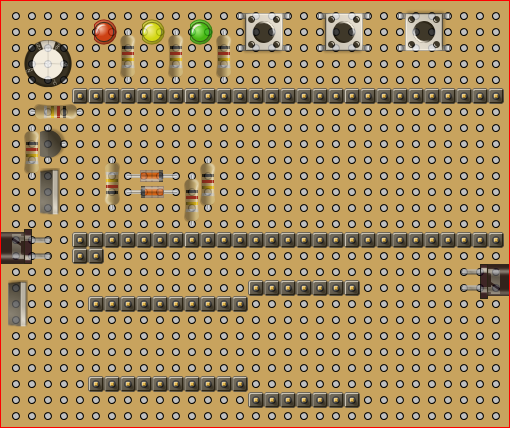
\includegraphics[width=260pt]{./picture/front.png}
        \caption{\label{lm324}{Vorderseite}}
    \end{figure}
    
    \begin{figure}[!ht]
    \centering
        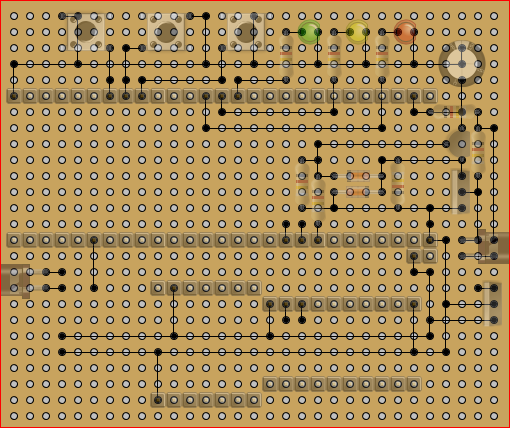
\includegraphics[width=260pt]{./picture/back.png}
        \caption{\label{lm324}{Rückseite}}
    \end{figure}


\section{Gehäuse}
Aufgrund eines vorhandenen 3D-Druckers konnte auch ein Gehäuse für den Prototypen umgesetzt werden.

\chapter{Zukunft}

\section{Software}
Eine anwenderfreundlichere Bediehnoberfläche ist zwingend notwendig. Weiters sollte eine Anwendung für die
mobile Benutzung entwickelt werden. Auch ein Command-Line Client wäre sinnvoll.

\section{Hardware}
Eine Erweiterung mit Funkmodulen für das 433kHz und das 844kHz Band wäre denkbar um auch die zahlreich vorhandenen
Geräte aus diesen Bereich steuern zu können. Nach dem Motto: ``One remote to control them all''

\section{Kommunikationstask}
Bla bla.... fsdfdsfds


 %\begin{figure}[!ht]
 %   \centering
 %       \includegraphics[width=260pt]{./picture/LM324_triangle.png}
        % LM324_triangle.png: 0x0 pixel, 250dpi, 0.00x0.00 cm, bb=
 %       \caption{\label{lm324}{Ausgangssignal LM324}}
 %   \end{figure}

%\restoregeometry

%\bibliographystyle{IEEEtran}
%\bibliography{Literatur}

% Abbildungsverzeichnis
% \listoffigures
% \addcontentsline{toc}{chapter}{Abbildungsverzeichnis} % f"ugt den Eintrag "Abbildungsverzeichnis" im Inhaltsverzeichnis hinzu
% % \newpage
%
% % Tabellenverzeichnis
% \listoftables
% \addcontentsline{toc}{chapter}{Tabellenverzeichnis} % f"ugt den Eintrag "Tabellenverzeichnis" im Inhaltsverzeichnis hinzu
% % \newpage

% Abk"urzungsverzeichnis
% Bei Verwendung der Dokumentklasse "scrartcl" ist der Befehlt \addchap{Abk"urzungsverzeichnis} durch
% \addsec{Abk"urzungsverzeichnis} zu ersetzen
\addchap{Abk"urzungsverzeichnis}
\hspace{-17mm}\begin{tabular}{>{\raggedleft}p{0.2\linewidth} p{0.75\linewidth} p{0.1\linewidth}}
PWM & Pulsweitenmodulation \\
OPV & Operationsverstärker
\end{tabular}

% Anh"ange
% \begin{appendix}
% \chapter[Erster Anhang]{Entwicklung und Aufbau eines Klasse D-Verstärkers}
% % \lhead{}
% % \lhead{\textcolor{blue}{\url{www.widatec.com/}}}\label{Anhang1}
% % \includepdf[pages={1-24},addtotoc={{24},{section},{2},{Entwicklung und Aufbau eines Klasse
% % D-Verstärkers},{D-Verstärker}}, pagecommand={\thispagestyle{fancy}},noautoscale=true,width=1.1\textwidth,offset=0cm
% % 1cm]{/home/christian/FH/3.Semester/ATK/Projekt/seminararbeit1/unterlagen/CAE.pdf}
% % \lhead{\studiumshort}
% %
%
% \chapter[Zweiter Anhang]{"Uberschrift des zweiten Anhangs}
%
% Text Text Text Text Text Text Text Text Text Text Text Text Text Text Text Text Text Text Text Text Text Text Text Text ...
%
% \end{appendix}

\end{document}
